\subsection{On confidence intervals}

Figure \ref{fig:ci} shows the impact of our diversion policy
for the 3 site case with a 60 minute lead time, by examining the
change of performance instead of simply the performance.
The confidence intervals show that the performance improvement
from our diversion policy is statistically
significant. Also, note that as we increase the fraction of
volunteers, the variance also increases. The reason is that,
when there are more volunteers, there are more diversions which
induce greater variance. If we examine the performance improvement
for other metrics or for other levels of granularity, similar patterns
can be observed.

\begin{figure}[htp]
\centering
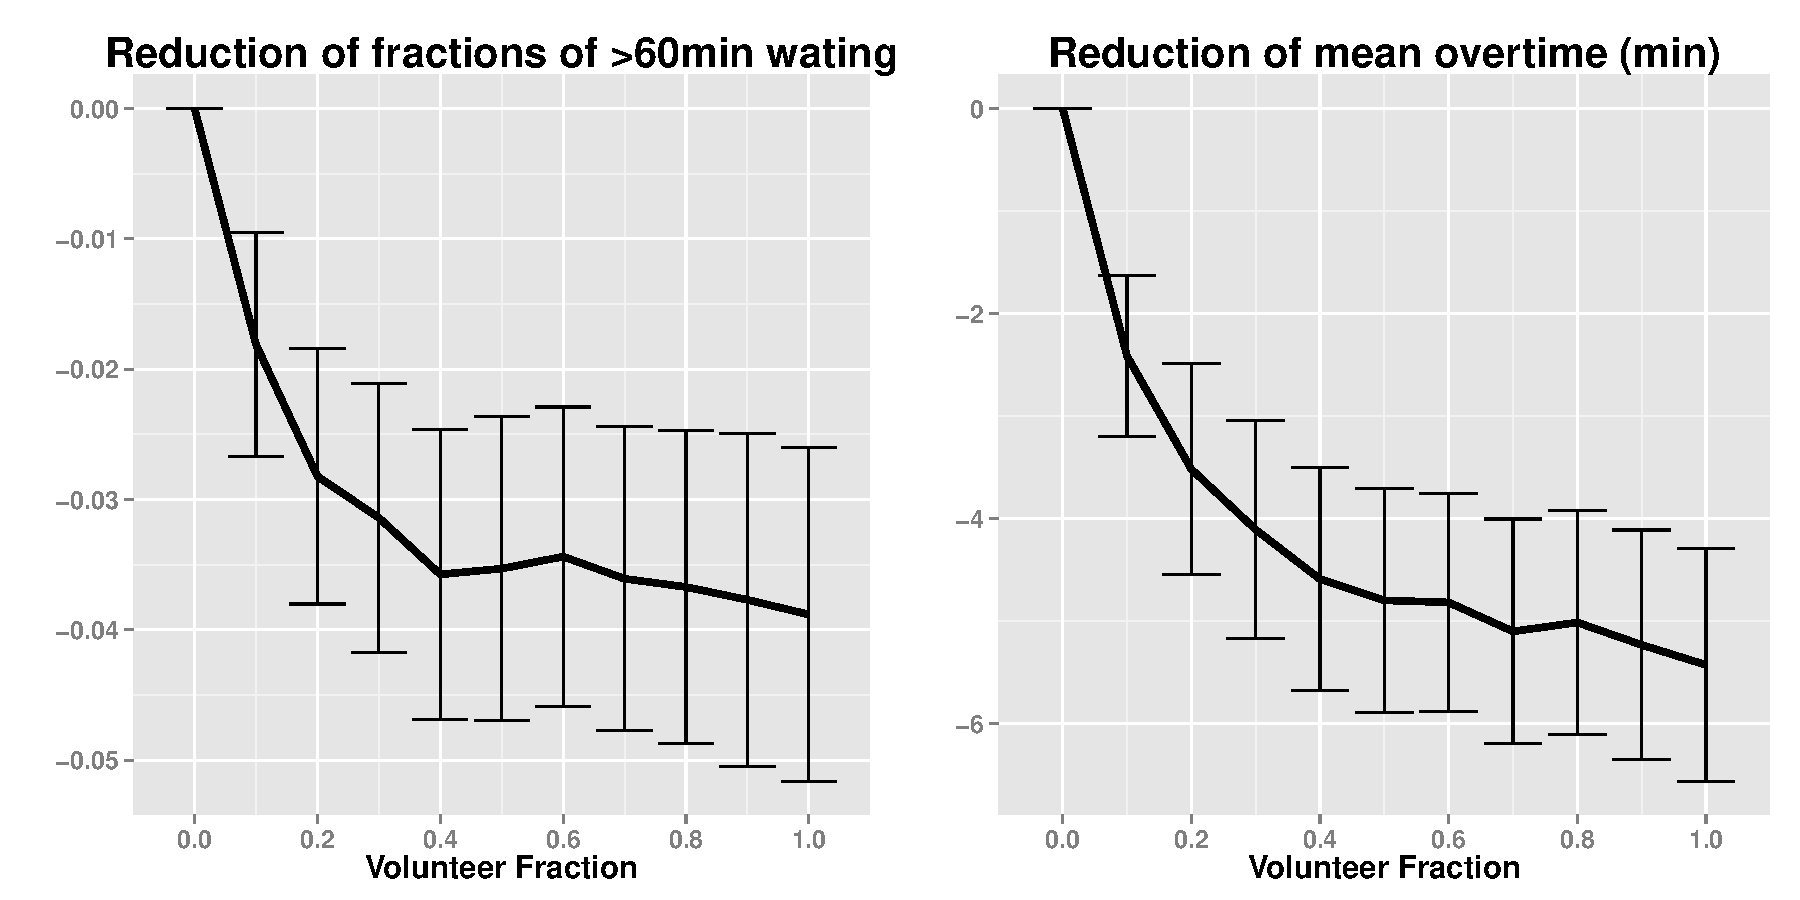
\includegraphics[width=.95\textwidth]{chap3/numeric/pic/ci}
\caption{The impact of diversion policy for the 3 site case
with a 60 minute lead time. The left plot is showing the
reduction of fractions of over 60 minute waiting. The right plot
is showing the reduction of mean overtime.}
\label{fig:ci}
\end{figure}

For more information, see Table
\ref{table:3site} and Table \ref{table:7site}.

% latex table generated in R 3.2.1 by xtable 1.8-0 package
% Tue Jan  5 14:10:23 2016
\begin{table}[ht]
\centering
\begin{tabular}{cccccc}
  \hline
  & Frac. of & Change of & Change of & Change of \\
Lead time & volunteers & $>$60min waiting \% & $>$90min waiting \% & overtime \\ 
  \hline
60 & 0.0 & 0.0\% +/- 0.0\% & 0.0\% +/- 0.0\% & 0.0 +/- 0.0 \\ 
  60 & 0.1 & -1.8\% +/- 0.3\% & -1.5\% +/- 0.2\% & -2.4 +/- 0.8 \\ 
  60 & 0.2 & -2.9\% +/- 0.4\% & -2.1\% +/- 0.3\% & -3.5 +/- 1.0 \\ 
  60 & 0.3 & -3.2\% +/- 0.4\% & -2.7\% +/- 0.3\% & -4.1 +/- 1.1 \\ 
  60 & 0.4 & -3.6\% +/- 0.5\% & -2.8\% +/- 0.3\% & -4.6 +/- 1.1 \\ 
  60 & 0.5 & -3.6\% +/- 0.5\% & -2.8\% +/- 0.3\% & -4.8 +/- 1.1 \\ 
  60 & 0.6 & -3.5\% +/- 0.5\% & -2.9\% +/- 0.3\% & -4.8 +/- 1.1 \\ 
  60 & 0.7 & -3.7\% +/- 0.5\% & -3.0\% +/- 0.3\% & -5.1 +/- 1.1 \\ 
  60 & 0.8 & -3.7\% +/- 0.5\% & -3.1\% +/- 0.3\% & -5.0 +/- 1.1 \\ 
  60 & 0.9 & -3.8\% +/- 0.5\% & -3.1\% +/- 0.3\% & -5.2 +/- 1.1 \\ 
  60 & 1.0 & -3.9\% +/- 0.5\% & -3.1\% +/- 0.3\% & -5.4 +/- 1.1 \\ 
  90 & 0.0 & 0.0\% +/- 0.0\% & 0.0\% +/- 0.0\% & 0.0 +/- 0.0 \\ 
  90 & 0.1 & -1.2\% +/- 0.3\% & -1.4\% +/- 0.2\% & -1.8 +/- 0.6 \\ 
  90 & 0.2 & -2.0\% +/- 0.4\% & -2.0\% +/- 0.3\% & -3.0 +/- 0.9 \\ 
  90 & 0.3 & -2.5\% +/- 0.4\% & -2.4\% +/- 0.3\% & -3.4 +/- 1.0 \\ 
  90 & 0.4 & -3.2\% +/- 0.4\% & -2.5\% +/- 0.3\% & -3.8 +/- 1.0 \\ 
  90 & 0.5 & -3.0\% +/- 0.4\% & -2.6\% +/- 0.3\% & -3.9 +/- 1.0 \\ 
  90 & 0.6 & -3.0\% +/- 0.4\% & -2.7\% +/- 0.3\% & -4.1 +/- 1.0 \\ 
  90 & 0.7 & -3.2\% +/- 0.5\% & -2.8\% +/- 0.3\% & -4.5 +/- 1.0 \\ 
  90 & 0.8 & -3.4\% +/- 0.5\% & -2.8\% +/- 0.3\% & -4.6 +/- 1.0 \\ 
  90 & 0.9 & -3.5\% +/- 0.5\% & -2.8\% +/- 0.3\% & -4.6 +/- 1.1 \\ 
  90 & 1.0 & -3.4\% +/- 0.5\% & -2.8\% +/- 0.3\% & -4.8 +/- 1.1 \\ 
   \hline
\end{tabular}
\caption{The performance improvement for 3 site case with confidence intervals.}
\label{table:3site}
\end{table}

% latex table generated in R 3.2.1 by xtable 1.8-0 package
% Tue Jan  5 14:10:23 2016
\begin{table}[ht]
\centering
\begin{tabular}{cccccc}
  \hline
  & Frac. of & Change of & Change of & Change of \\
Lead time & volunteers & $>$60min waiting \% & $>$90min waiting \% & overtime \\ 
  \hline
  60 & 0.0 & 0.0\% +/- 0.0\% & 0.0\% +/- 0.0\% & 0.0 +/- 0.0 \\ 
  60 & 0.1 & -2.0\% +/- 0.4\% & -2.2\% +/- 0.3\% & -4.9 +/- 1.0 \\ 
  60 & 0.2 & -3.0\% +/- 0.5\% & -3.7\% +/- 0.4\% & -7.3 +/- 1.1 \\ 
  60 & 0.3 & -4.2\% +/- 0.5\% & -4.8\% +/- 0.4\% & -8.5 +/- 1.3 \\ 
  60 & 0.4 & -4.9\% +/- 0.6\% & -5.3\% +/- 0.5\% & -9.6 +/- 1.4 \\ 
  60 & 0.5 & -5.0\% +/- 0.6\% & -5.7\% +/- 0.5\% & -10.2 +/- 1.4 \\ 
  60 & 0.6 & -5.2\% +/- 0.6\% & -5.9\% +/- 0.5\% & -10.4 +/- 1.4 \\ 
  60 & 0.7 & -5.8\% +/- 0.6\% & -6.0\% +/- 0.5\% & -10.7 +/- 1.4 \\ 
  60 & 0.8 & -6.2\% +/- 0.6\% & -6.5\% +/- 0.5\% & -11.2 +/- 1.5 \\ 
  60 & 0.9 & -6.6\% +/- 0.7\% & -6.8\% +/- 0.5\% & -11.6 +/- 1.4 \\ 
  60 & 1.0 & -6.7\% +/- 0.7\% & -6.9\% +/- 0.5\% & -11.9 +/- 1.5 \\ 
  90 & 0.0 & 0.0\% +/- 0.0\% & 0.0\% +/- 0.0\% & 0.0 +/- 0.0 \\ 
  90 & 0.1 & -1.3\% +/- 0.4\% & -1.7\% +/- 0.3\% & -3.9 +/- 0.9 \\ 
  90 & 0.2 & -2.3\% +/- 0.5\% & -3.3\% +/- 0.4\% & -6.1 +/- 1.1 \\ 
  90 & 0.3 & -3.5\% +/- 0.5\% & -4.1\% +/- 0.4\% & -7.7 +/- 1.2 \\ 
  90 & 0.4 & -4.0\% +/- 0.5\% & -4.8\% +/- 0.5\% & -8.3 +/- 1.3 \\ 
  90 & 0.5 & -4.0\% +/- 0.6\% & -5.2\% +/- 0.5\% & -8.7 +/- 1.3 \\ 
  90 & 0.6 & -4.2\% +/- 0.6\% & -5.2\% +/- 0.5\% & -9.5 +/- 1.4 \\ 
  90 & 0.7 & -4.6\% +/- 0.6\% & -5.5\% +/- 0.5\% & -9.6 +/- 1.4 \\ 
  90 & 0.8 & -4.8\% +/- 0.6\% & -5.8\% +/- 0.5\% & -10.0 +/- 1.4 \\ 
  90 & 0.9 & -5.0\% +/- 0.6\% & -6.1\% +/- 0.5\% & -10.4 +/- 1.4 \\ 
  90 & 1.0 & -5.0\% +/- 0.6\% & -6.5\% +/- 0.5\% & -10.6 +/- 1.4 \\ 
   \hline
\end{tabular}
\caption{The performance improvement for 7 site case with confidence intervals.}
\label{table:7site}
\end{table}
